\chapter{Gold standard}
\label{chap:gold-standard}
\section{Introduction}
In the previous chapter, I discussed SimAlign, a method for computing word alignment based on measuring similarity between multilingual word embeddings. 
The clear advantage of this method is that it does not rely on the existence of large amounts of parallel data. 
The multilingual word embeddings can be learned from monolingual data. 
\cite{jalili-sabet-etal-2020-simalign} evaluated their method on language pairs which were all part of the training data for the language models in use (mBERT and XLM-R). 
In the course of this work, I was able to extract \numprint{79109} sentence pairs for German-Romansh. 
I shall now proceed to test how well SimAlign performs on this language pair, considering the fact the Romansh wasn't included in the training data for these models. 


In order to measure the quality of words alignments, a model's performance is measured on a test set which is a gold standard created by human annotators. 
For the gold standard to be of good quality and consistent with itself, annotators have to follow strict guidelines.
These guidelines address issues of ambiguity in word alignments. \autocite[115]{koehn2009}. 

Some problematic cases that might occur are function words (TODO) that have no clear equivalent in the other language. 
\cite{koehn2009} gives as an example the German-English sentence pair: \emph{John wohnt hier nicht}  \emph{John does not live here}. 
What German word should the English word \emph{does} be aligned to? 
Three different choices can be made:
\begin{enumerate}
	\item The word should remain unaligned since it has to clear equivalent in German.
	\item The word \emph{does} is connected with \emph{live}; it contains the number and tense information which is in German contained in one word \emph{wohnt}, so it should be aligned to \emph{wohnt}, together with \emph{live}.
	\item \emph{does} is part of the negation; without it, the sentence would not contain this word. Therefore, \emph{does} should be aligned with \emph{nicht} (the German negation).
\end{enumerate}

\section{Sure and Possible Alignments}
\label{sec:sure_possible}
An approach for solving problematic cases is the distinction between \emph{sure} (s) and \emph{possible} (p) alignments \autocite{och-ney-2000-improved}, which are also sometimes referred as fuzzy alignments \autocite{clematide2018}. 
Generally, these labels allow to distinguish between ambiguous and unambiguous links. 
Ambiguous links are labeled \emph{possible} and unambiguous links are labeled \emph{sure} \autocite{lambert2005}. 
The \emph{possible} label was conceived to be used especially for aligning words within idiomatic expressions, free translations and missing function words \autocite{och-ney-2000-improved}.
This distinction also has an impact on the way the evaluation metrics are computed (more on that later).

There seems to be no clear global definition about which alignments should be considered as umabiguous and marked as \emph{sure} and which should be considered ambiguous marked as \emph{possible}. 
For some created gold standards, no distinciton between \emph{sure} and \emph{possible} alignments was made \autocite{clematide2018}. 
In another case, annotators were asked to first label all alignments as \emph{sure} and then refine their alignments with confidence labels \autocite{holmqvist-ahrenberg-2011-gold}. 
In the creation of the English-Icelandic gold standard in \cite{steingrimsson-etal-2021-combalign},  annotators used only \emph{sure} links. 
Their annotations were then combined, with all 1-1 alignments both annotators agreed upon (i.e., the intersection of their annotations) makred as \emph{sure} and differences all other alignments made by either one or both were marked as \emph{possible} \autocite{steingrimsson-etal-2021-combalign}. 

\section{Evaluation Metrics}
TODO: move to results/evaluation part
Four types of measures have become standard for evaluating word alignment. Three of them -- precision, recall and F-measure -- are well known in Information Retrieval metrics \cite{mihalcea-pedersen-2003-evaluation}. 
The fourth, alignment error rate (AER) one was introduced by \cite{och-ney-2000-improved}.

\section{Gold standard for German-Romansh}
In order to measure the performance of both models, the embedding based model (SimAlign) and the stastitical model (fast\_align), on the language pair German-Romansh a gold standard is needed. 
Since no such gold standard exists, I took upon myself to create one. 
Although I am not a speaker of Romansh, my experience as a trained linguist, as well as my knowledge in related languages (Latin, Italian, French), allows me to confidently tackle this task. 
Additionally, whenever I was in doubt, I referred to the online dictionary \href{https://www.pledarigrond.ch/rumantschgrischun}{Pledari grond}, which also offers a grammar overview. 
(TODO: add more grammar references)

\subsection{Annotation tool}
\label{sec:AlignMan}
I used the tool \emph{AlignMan} which was originally programmed for creating the gold standard for English-Icelandic by \cite{steingrimsson-etal-2021-combalign}. 
It is quite easy to use and its code is readable. 
I also had to make some small changes to the code. 
For instance, the sentences to be aligned, while loaded into the database, were read in opposite order, such that the source language became the target language and vice versa. 
I fixed this issue, so that source (German) and target (Romansh) languages stay the same accross all applications.

As mentioned above, the tool does not allow labeling of links with \emph{Sure} and \emph{Possible}. 
Instead, AlignMan treats the union of 1-1 alignments made by two annotators as \emph{Sure} alignments and all other alignments as \emph{Possible}. 
This means, each annotator is expected to only annotate \emph{Sure} alignments, which also applied to me while annotating the German-Romansh gold standard. 


\subsection{Guidelines}
As mentioned above, clear guidelines need to be defined for creating the gold standard in order to ensure quality and consistency. I shall now proceed to describe the guidelines I used for my annotation of the word alignments for the gold standard.

A motto cited often for annotating word alignments is \enquote{Align as small segments as possible, and as long segments as necessary} (\cite{Vronis00evaluationof}, cited in \cite{lines2007}). A variation of this is found in \cite{clematide2018}: \enquote{as few words as possible and as many words as necessary that carry the same meaning should be aligned.}, referring to \cite{lambert2005}. 

In the following sections I will list some general principles as well as more specific principles involving German and Romansh.

\subsection{General priniciples}
\paragraph{Principle I.} 
Use only \emph{Sure} alignments. 
Since the annotating tool I was using does not provide the use of confidence labels (cf.~section~\ref{sec:AlignMan}), I only aligned words which would be considered \emph{Sure} alignments, i.e., they are unambiguous (cf.~section~\ref{sec:sure_possible}). 


\paragraph{Principle II.}
Prefer 1-1 alignments over 1-n alignments or n-n alignments. 
Since all alignments are seen as \emph{Sure} alignments, 1-n alignments should be avoided, unless a single word in the source sentence lexically corresponds to several words in the target sentence (see TODO principle sth.)
This means alignments of phrases should be avoided. This is also due to the fact that we are testing models for automatic word, and not phrase alignments.

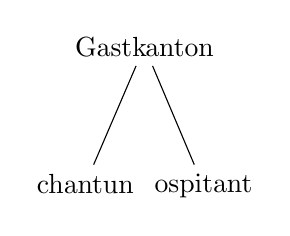
\begin{tikzpicture}
\node[align=left, anchor=north]{Gastkanton}
	child { node[anchor=north]{chantun}}
	child { node[anchor=north]{ospitant}}
;
\end{tikzpicture} 

Words that are repeated in one language, but not in the other, should only be linked once, leaving the repetition unaligned.

\paragraph{Principle III.}
Lexical alignments should always be preferred over all other alignments (part-of-speech alignments or morphosyntactical alignments). 
This means alignments should describe first and foremost lexical correspondences, i.e., they have the same lexical meaning (but not necessarily share the same grammatical function or the same part-of-speech).
Only words that are translations of each other also outside of the specific context of the sentence pair at hand should be aligned. This is in line with \cite{clematide2018}.
In cases of paraphrasing during translations, words should remain unaligned (TODO: example?)

\begin{itemize}
	\item only sure alignments
	\item prefer 1-1 alignments over 1-n alignments
	\item align words, not phrases
	\item only align words that are translations of each other also outside of context
	\item POS doesn't matter: German often prefers a nominal style, Romansh prefers a verbal style -- expect some noun-verb alignments.

\end{itemize}

\subsection{Examples}
I will now supply some examples to illustrate the above principles.
\subsubsection{Compound words}
Compounding is the formation of new lexemes by adjoining two or more lexemes \autocite{bauer1988}. In German, compounds are productive and prominent means of word formation in German \autocite{clematide2018}. 
In a sample of 4,500 types examined by \cite{clematide2018}, 80\% of German nouns were compounds.
Romansh, in comparison, uses prepositions (usually \emph{da}) for linking nouns, with one noun modifying the other \autocite{valladers}. Other prepositions that can be found for linking words are \emph{cunter} and \emph{per}.
\footnote{Typologically, this is inline with other Romance languages such as French, which uses prepositions (\emph{de}, \emph{en} and \emph{à}) for linking two nouns, e.g., \emph{une robe de soie} \enquote{a silk dress} \autocite{price2008}[510].}
In other cases, German compounds might be translated to Romansh using an adjective + noun, e.g., German \emph{Gastkanton} was translated to \emph{chantun ospitant} ~\enquote{hosting canton}.
See table~\ref{tab:compounds} for examples.

\textbf{German compounds will be aligned to their equivalent lexical words, but not to function words, resulting in a 1-n alignment}: \emph{Webseite} \textasciitilde  \emph{pagina [d'] internet}, \emph{Gebäudeversicherung} \textasciitilde \emph{Assicuranza [d'] edifizis}. 
This is also inline with principles I, II and III in \cite{clematide2018}.

\begin{table}
	\begin{center}
	\begin{tabular}{lll}
		\toprule
		German & Romansh &  \\
		\midrule
		\emph{Beratungsstelle} & \emph{post \textbf{da} cussegliaziun} & \enquote{consultation point} \\
		\emph{Gebäudeversicherung} & \emph{Assicuranza \textbf{d}'edifizis} & \enquote{building insurance} \\
		\emph{Webseite} & \emph{pagina \textbf{d}'internet} & \enquote{web site} \\
		\emph{Kindermasken} & \emph{mascrinas \textbf{per} uffants} & \enquote{children masks} \\
		\emph{Brandversicherung} & \emph{assicuranza \textbf{cunter} fieu} & \enquote{fire insurance} \\
		\emph{Gastkanton} & \emph{chantun ospitant} & \enquote{hosting canton} \\
		\bottomrule
	\end{tabular}
	\caption{Translation examples of German compounds into Romansh}
	\label{tab:compounds}
	\end{center}
\end{table}

\subsubsection{German preterite vs.~Romansh perfect}
In the corpus at hand, two tenses are used in German for referring to past events: the preterite and the perfect. 
The German preterite is a synthetic verb form, i.e., it is made up of a single conjugated form. 
Some examples are \emph{nahm} (infinitive \emph{nehmen} \enquote{take}) or \emph{wurde} (infinitive \emph{werden} \enquote{become}). 
The German perfect is an analytic construction made up of an auxiliary verb (\emph{haben} \enquote{have} or \emph{sein} \enquote{be}) and the past participle, e.g., \emph{Die Präsidentenkonferenz \textbf{hat} nun \textbf{entschieden}} \enquote{The conference has decided}. 

In contranst to German, Romansh only has one tense referring to past events: the perfect. 
It is an analytic construction made, in a similar fashion as in German, of an auxiliary \emph{habere} \enquote{have} for transitive verbs or \emph{esse} \enquote{be} for intransitive verbs and the past participle \autocite[189]{bossong2008}. 
The German sentence given above (\emph{Die Präsidentenkonferenz hat nun entschieden}) was translated as \emph{La conferenza da las presidentas e dals presidents \textbf{ha} usse \textbf{decidi}}. 
\emph{ha} is the auxiliary and \emph{decidi} is the past participle. 
This poses no real problem since we can link the German auxiliary to the Romansh auxiliary and the German participle to the Romansh participle.

\begin{figure}
\centering
        \tikzmarknode{DIE}{Die} \tikzmarknode{PRAES}{Präsidentenkonferenz} \tikzmarknode{HAT}{hat} \tikzmarknode{ENT}{entschieden} 
        
        \vspace*{1cm}
        
        \tikzmarknode{LA}{La} \tikzmarknode{CON}{conferenza} \tikzmarknode{de}{de} \tikzmarknode{LAS}{las} \tikzmarknode{PRESIDENTAS}{presidentas} 
        \tikzmarknode{E}{e} \tikzmarknode{DALS}{dals} \tikzmarknode{PRESIDENTS}{presidents} \tikzmarknode{HA}{ha} \tikzmarknode{DECIDI}{decidi}

    
    \begin{tikzpicture}[remember picture, overlay]
        \draw    (DIE) -- (LA)
                (PRAES.south) -- (PRESIDENTS)
                (PRAES.south) -- (CON)
                (HAT.south) -- (HA.north)
                (ENT) -- (DECIDI);
    \end{tikzpicture}
\caption{Aligning German perfect to Romansh perfect}
\end{figure}


\begin{figure}
\centering
\tikzmarknode{s0}{Der} \tikzmarknode{s1}{Kanton} \tikzmarknode{s2}{Graubünden} \tikzmarknode{s3}{war} \tikzmarknode{s4}{letztmals} \tikzmarknode{s5}{2003} \tikzmarknode{s6}{Gastkanton} \tikzmarknode{s7}{.}

\vspace*{1cm}

\tikzmarknode{t0}{Il} \tikzmarknode{t1}{chantun} \tikzmarknode{t2}{Grischun} \tikzmarknode{t3}{è} \tikzmarknode{t4}{stà} \tikzmarknode{t5}{l'} \tikzmarknode{t6}{ultima} \tikzmarknode{t7}{giada} \tikzmarknode{t8}{l'} \tikzmarknode{t9}{onn} \tikzmarknode{t10}{2003} \tikzmarknode{t11}{chantun} \tikzmarknode{t12}{ospitant} \tikzmarknode{t13}{.}
\begin{tikzpicture}[remember picture, overlay, scale=0.6, every node/.style={scale=0.6}]
\draw
(s0) -- (t0)
(s1) -- (t1)
(s2) -- (t2)
(s3) -- (t4)
(s4) -- (t6)
(s4) -- (t7)
(s5) -- (t10)
(s6.south) -- (t11)
(s6.south) -- (t12)
(s7) -- (t13)
;
\end{tikzpicture}
\caption{Alignment of German preterite to Romansh perfect}
\label{fig:pret-perf}
\end{figure}

However, a German preterite is always translated using the Romansh perfect. 
For example, in the sentence \emph{Der Kanton Graubünden war letzsmals 2003 Gastkanton} \enquote{The last time the Canton of Grisons was a host canton was in 2003} the verb \emph{war} \enquote{was} is translated as \emph{è stà}. 
This theoretically results in a 1-2 link. 
However, since the verb \emph{è} here only carries grammatical information of tense and number, but no real lexical information, it should reamin unaligned. 

\textbf{The German perfect should be aligned to the Romansh perfect using a 1-1 alignment}; auxiliary to auxiliary and participle to participle. 
\textbf{The German preterite should also be aligned using a 1-1 alignment to the Romansh participle, leaving the auxiliary unaligned and avoiding a 1-2 alignment.}

\subsubsection{German present participle}
German present participles (known in German as \emph{Partizip I}) are translated to Romansh using relative clauses. Moreover, adjectives (and participles in the function of adjectives), can be nominalized, meaning they become the head of a noun phrase and there is no need for an actual noun. 
A good example for that in the corpus is the German noun phrase \emph{nichtarbeitslose Stellensuchende} (cf. ex.~\ref{ex:stellensuchende}), which was translated as a noun phrase with a relative clause: \emph{persunas che tschertgan ine plazza che n'èn betg dischoccupadas} \enquote{persons who look for a job who are not unemployed}.

\begin{exe}
   \ex\label{ex:stellensuchende} 
   \gll nicht-arbeit-s-los-e Stellen-such-end-e  \\
        not-work-\textsc{gen}-less-\textsc{Pl} job-search-\textsc{pres.part}-\textsc{pl} \\
        \trans \enquote{People looking for jobs who are not unemployed}
\end{exe}

\begin{figure}
\centering
\tikzmarknode{s3}{nichtarbeitslose} \tikzmarknode{s4}{Stellensuchende} \

\vspace*{1cm}

\tikzmarknode{t7}{persunas} \tikzmarknode{t8}{che} \tikzmarknode{t9}{tschertgan} \tikzmarknode{t10}{ina} \tikzmarknode{t11}{plazza} \tikzmarknode{t12}{che} \tikzmarknode{t13}{n'} \tikzmarknode{t14}{èn} \tikzmarknode{t15}{betg} \tikzmarknode{t16}{dischoccupadas} \tikzmarknode{t17}{.}
\begin{tikzpicture}[remember picture, overlay, scale=0.6, every node/.style={scale=0.6}]
\draw
(s3.south) -- (t15.north)
(s3.south) -- (t16)
(s4.south) -- (t11)
(s4.south) -- (t9)
;
\end{tikzpicture}
\caption{Aligning German present participles to Romansh relative clauses}
\end{figure}

In this case, these two phrases should not be aligned as phrases, but only the content words which lexically correspond to each other: \emph{nichtarbeitslose} \textasciitilde ~ \emph{betg dischoccupadas}; \emph{Stellensuchende} \textasciitilde ~\emph{tschertgan [ina] plazza}.

\subsubsection{Double negation}
Negation in Romansh is built using two particles: \emph{na} and \emph{betg} to negate verbs or \emph{nagin-} to negate nouns. 
Since we prefer 1-1 alignments, the German negations \emph{nicht} (for verbs) and \emph{kein-} for nouns should be aligned only to the second Romansh particle (\emph{betg}/\emph{nagin-}), leaving Romansh \emph{na} unaligned. 
Granted, this is also in favor of the SimAlign output, but it is also linguistically motivated: when negating the imperative form, \emph{na} can be omitted required TODO:cite Grammatica per l’instrucziun dal rumantsch grischun. 

\subsubsection{Articles and prepositions}
German articles inflect in case, which expresses some syntactic relations between nouns. 
Romansh often uses preopsitions for expressing the same relations. 
For instance \emph{Zustimmung der Person} \enquote{the person's agreement} is translated as \emph{consentiment da la persuna}. 
I align the German article \emph{der} with Romansh \emph{da}, leaving \emph{la} unaligned. 
Except for my preference for 1-1 alignments, the motivation for this is that it is the preposition \emph{da} that expresses the genitival relations between the nouns.

\subsubsection{Separable verbs}
German uses many verbs to which an adverb or a preopisition is affixed in order to delimit the verb's meaning (or sometimes completely change its meaning). 
In such cases, both the verb and its affix should be aligned to the corresponding Romansh verb, resulting in a 2-1 alignment.

\section{Flaws}
I shall now discuss the quality of my gold standard and some flaws it has.

The most obvious flaw is the fact that I created the gold standard alone. 
With more than one annotator, more intricate annotating schemes can be used in order to ensure higher quality, consistency and harmony. 
For instance the annotators' agreement can be measured using the so-called inner-annotator agreement \autocite{holmqvist-ahrenberg-2011-gold}. 
Further, the intersection of the annotators' \emph{Sure} alignment can be used to build the final \emph{Sure} alignments set and the reunion of the \emph{Possible} alignments can be used to create the final \emph{Possible} alignments set \cite{mihalcea-pedersen-2003-evaluation}.
A third annotator can also revise and resolve conflicts between two annotaors \cite{mihalcea-pedersen-2003-evaluation}.
When several annotators work on the same task, they can also discuss conflicts and resolve them using a majority vote \autocite{DBLP:journals/corr/cmp-lg-9805004}.

All of these possible schemes cannot be realized in my case.

Another flaw is the missing confidence labels (\emph{Sure} and \emph{Possible}), which may influence the evaluation scores. 
Doing without \emph{Possible} links and using only \emph{Sure} links is however precedented \autocites{clematide2018,mihalcea-pedersen-2003-evaluation} and hence defensible.

In order to test my own consistency, I have re-annotated the first 100 sentences in the sample. 
TODO: results

Despite of the flaws mentioned, I am certain that gold standard is of high quality and consistency, due to the fact that I was also the one to define the guidelines.

